\documentclass[12pt,a4paper,notitlepage,fleqn,twoside]{book}		% Zweiseitiger Druck
%\documentclass[12pt,a4paper,notitlepage,fleqn,oneside]{book}		% Einseitiger Druck

%%%%%%%%%%%%%%%%%%%%%%%%%%%%%%%%%%%%%%%%%%%%%%%%%%%%%%%%%%%%%%%%%%%%%%%%%%%%%%%%%%%%%%%%%%%%%%%%%%%%%%%%
%%%   Bitte Ueberpruefen!!!	                                                                       %%%
%%%%%%%%%%%%%%%%%%%%%%%%%%%%%%%%%%%%%%%%%%%%%%%%%%%%%%%%%%%%%%%%%%%%%%%%%%%%%%%%%%%%%%%%%%%%%%%%%%%%%%%%

% Ein- oder zweiseitiger Druck - Documentclass oben entsprechend anpassen!
%\newcommand{\Drucklayout}{Einseitig}
\newcommand{\Drucklayout}{Zweiseitig}

% Fuer serifenlose Schrift folgendes einkommentieren
%\newcommand{\Schriftart}{serifenlos}
\newcommand{\Schriftart}{LaTeX-Standard}


%%%%%%%%%%%%%%%%%%%%%%%%%%%%%%%%%%%%%%%%%%%%%%%%%%%%%%%%%%%%%%%%%%%%%%%%%%%%%%%%%%%%%%%%%%%%%%%%%%%%%%%%
%%%   Packages, eigene Makros und Formatdefinitionen                                                 %%%
%%%%%%%%%%%%%%%%%%%%%%%%%%%%%%%%%%%%%%%%%%%%%%%%%%%%%%%%%%%%%%%%%%%%%%%%%%%%%%%%%%%%%%%%%%%%%%%%%%%%%%%%

	
\usepackage[english,german]{babel} 	% Sprachpaket
% \usepackage[latin1]{inputenc} 		% Konvertierungspaket (Sprachen:Westeuropa)
\usepackage[utf8]{inputenc} 		% joba Konvertierungspaket (Sprachen:Westeuropa)

\usepackage[centertags]{amsmath}		% Mathepakete
\usepackage{amssymb}
\usepackage{array}

\usepackage{eso-pic}
\usepackage[pdftex]{graphicx}
\usepackage{epstopdf}

\usepackage[absolute]{textpos}

\usepackage[format=hang, font=footnotesize, labelfont=bf]{caption}  % Layout fuer Bildbeschriftung

\usepackage{fancyhdr}	% Definition von Kopf- und Fusszeilen

\usepackage{color}		% fuer farbige Texte

\usepackage{calc}

%\usepackage{tocstyle}	% Package fuer Layout des Inhaltsverzeichnisses
\usepackage{tocloft}	% Package zum Bearbeiten des Layouts des Abbildungs- und Tabellenverzeichnisses
\usepackage{titletoc}	% Package zum Bearbeiten des Layouts des Inhaltsverzeichnisses

\normalsize

%-----------------------------------------------------------------------------------------------------------%

\usepackage{textcomp}

\usepackage{subcaption}	% Subcaptions

\usepackage{multirow}	% Multirow - Tabellen
\usepackage{longtable}	% Lange Tabelle

\usepackage{color}		% fuer Farben im allgemeinen
\usepackage{colortbl}	% fuer die Hintergrundfarbe einzelner Zellen in Tabellen

\usepackage{url}		% URL-Package

\usepackage{ifthen}		% if then
\usepackage{nomencl}	% Abkuerzungen und Verzeichnisse
\usepackage{makeidx}	% Index erstellen

\usepackage{blindtext}	% Lorem ipsum

\usepackage[]{hyperref}	% Links usw.

\usepackage{setspace}	% Zeilenabstand

\usepackage[bottom]{footmisc}	% Fussnotenposition
\usepackage{chngcntr}

\usepackage{pdfpages}

\ifthenelse{\equal{\Schriftart}{serifenlos}}{
	\usepackage[scaled=0.92]{helvet}
	\renewcommand{\familydefault}{phv}
}{}


			% Notwendige Packete
	
% Makros
\newcommand{\VECSYM}[1]{\boldsymbol{#1}}			% Symbol als Vektor (fett)
\newcommand{\VEC}[1]{\mathbf{#1}}					% Vektor (fett)
\newcommand{\sign}[1]{\mbox{sign}\left\{#1\right\}}	% Signum-Funktion
\newcommand{\intd}{\textnormal{\;d}}				% d bei einem Integral
\newcommand{\ind}[1]{_\textnormal{#1}}				% konstanter Index in Matheumgebung (nicht kursiv)
\newcommand{\einheit}[1]{\,\textnormal{#1}}			% Einheit in Matheumgebung (nicht kursiv)
\newcommand{\const}[1]{\textnormal{#1}}				% Konstante in Matheumgebung (nicht kursiv)


% Aufz�hlungs-Umgebungen
\newenvironment{einszweidrei}{\begin{enumerate}\renewcommand{\labelenumi}{\arabic{enumi}.}}{\end{enumerate}}
\newenvironment{iii}{\begin{enumerate}\renewcommand{\labelenumi}{\roman{enumi})}}{\end{enumerate}}


% Farben
\definecolor{dunkelgrau}{rgb}{0.8,0.8,0.8}
\definecolor{hellgrau}{rgb}{0.9,0.9,0.9}


% Rechtsb�ndige Spalten mit fester Breite
\newcolumntype{R}[1]{>{\raggedleft\arraybackslash}p{#1}}			% Selbstdefinierte Befehle
	\hoffset-1in
\voffset-1in

\evensidemargin2cm
\textwidth16cm
\setlength{\oddsidemargin}{21cm - \textwidth - \evensidemargin}
\topmargin2cm
\headheight.7cm
\headsep.8cm
\topskip12pt
\textheight22.8cm
\footskip1.2cm
\renewcommand{\baselinestretch}{1.25}
\unitlength1cm


\setlength{\mathindent}{1cm}
\newlength{\matfigwidth}
\setlength{\matfigwidth}{12cm}
\newlength{\figheight}
\setlength{\figheight}{10cm}
\setlength{\abovecaptionskip}{10pt}

\captionsetup{width=.95\textwidth}

% Einstellung des Absatzes
\parskip1ex plus .2ex minus .2ex % zus�tzlicher Abstand
\parindent0pt % Einzug

\frenchspacing % Ausschalten des Zusatzzwischenraums nach Satzzeichen

\pagestyle{fancy}
\fancyhead{}
\fancyfoot{}
\renewcommand{\headrulewidth}{0pt}
\renewcommand{\footrulewidth}{0pt}

\fancypagestyle{plain}{
    \fancyhf{}
    \renewcommand{\headrulewidth}{0pt}
    \renewcommand{\footrulewidth}{0pt}
}

\setcounter{secnumdepth}{3} % 3 Gliederungsebenen im laufenden Text

\sloppy % Laesst unguenstige Zeilenumbrueche bei schmalen Spalten zu			% Allgemeines Format der Arbeit
	

%%%%%%%%%%%%%%%%%%%%%%%%%%%%%%%%%%%%%%%%%%%%%%%%%%%%%%%%%%%%%%%%%%%%%%%%%%%%%%%%%%%%%%%%%%%%%%%%%%%%%%%%
%%%   Titel, Art der Arbeit,Bearbeiter und Abgabedatum                                               %%%
%%%%%%%%%%%%%%%%%%%%%%%%%%%%%%%%%%%%%%%%%%%%%%%%%%%%%%%%%%%%%%%%%%%%%%%%%%%%%%%%%%%%%%%%%%%%%%%%%%%%%%%%

	\newcommand{\TITEL}{Titel der Arbeit, welcher über zwei Zeilen gehen sollte}
	\newcommand{\ARBEIT}{Diplomarbeit}
	\newcommand{\STUDIENGANG}{Elektrotechnik-Elektronik-Informationstechnik}
	\newcommand{\NAME}{Vorname Nachname}
	\newcommand{\MATRNR}{123456789}
	\newcommand{\BEARBEITUNGSZEIT}{x}			% in Monaten
	\newcommand{\ENDE}{01.07.2012}
	\newcommand{\TITELBILD}{StudArbeitenTitelbildVorlage}


%%%%%%%%%%%%%%%%%%%%%%%%%%%%%%%%%%%%%%%%%%%%%%%%%%%%%%%%%%%%%%%%%%%%%%%%%%%%%%%%%%%%%%%%%%%%%%%%%%%%%%%%
%%%   Bitte Ueberpruefen!!!	                                                                       %%%
%%%%%%%%%%%%%%%%%%%%%%%%%%%%%%%%%%%%%%%%%%%%%%%%%%%%%%%%%%%%%%%%%%%%%%%%%%%%%%%%%%%%%%%%%%%%%%%%%%%%%%%%


% Pfad der Bilder
\graphicspath{{./Bilder/}}

% Nur Abkuerzungsverzeichnis (bzw. danach Symbolverzeichnis)
\newcommand{\Verzeichnisse}{AbkuerzungSymbol}

% Nur Symbolverzeichnis
%\newcommand{\Verzeichnisse}{Symbol}

% Lebenslauf
\newcommand{\Lebenslauf}{noCV}	% kein Lebenslauf notwendig
%\newcommand{\Lebenslauf}{CV}		% Lebenslauf am Ende der Arbeit


% TODO: joba auskommentiert da Probleme beim auto-build
% TODO: ML funktioniert unter TeXnicCenter 2.02 Stable (64 bit)
% Einstellungen fuer Hyperlinks usw. 
\ifthenelse{\equal{\Drucklayout}{Zweiseitig}}{
	\hypersetup{
		hidelinks,
		pdfdisplaydoctitle=true,
		pdfstartview={Fit},
		pdfpagelayout=TwoPageRight,
		pdfinfo={
			Title={\TITEL},
			Author={\NAME},
			Subject={\ARBEIT}
		}
	}
}{
	\ifthenelse{\equal{\Drucklayout}{Einseitig}}{
		\hypersetup{
			hidelinks,
			pdfdisplaydoctitle=true,
			pdfstartview={Fit},
			pdfpagelayout=SinglePage,
			pdfinfo={
				Title={\TITEL},
				Author={\NAME},
				Subject={\ARBEIT}
			}
		}
	}{}
}



%%%%%%%%%%%%%%%%%%%%%%%%%%%%%%%%%%%%%%%%%%%%%%%%%%%%%%%%%%%%%%%%%%%%%%%%%%%%%%%%%%%%%%%%%%%%%%%%%%%%%%%%
%%%   Abkuerzungen				                                                                  %%%
%%%%%%%%%%%%%%%%%%%%%%%%%%%%%%%%%%%%%%%%%%%%%%%%%%%%%%%%%%%%%%%%%%%%%%%%%%%%%%%%%%%%%%%%%%%%%%%%%%%%%%%%


% Abkuerzungen bzw. Verzeichnisse
	\let\abk\nomenclature
	
%	\renewcommand{\nomlabel}[1]{#1 \dotfill}	% Punkte zw. Abkuerzung und
% Erklaerung
	\setlength{\nomlabelwidth}{2.0cm} 			% Abstand zwischen Abkuerzung und Erklaerung
	\setlength{\nomitemsep}{-0.5pc}			% Zeilenabstaende verkleinern


\ifthenelse{\equal{\Verzeichnisse}{AbkuerzungSymbol}}{

	%%%%%%%%%%%%%%%%%%%%%%%%%%%%%%%%%%%%%%%%%%%%%%%%%%%%%%%%%%%%%%%%%%%%%%%%%%%%%%%%%%%%%%%%%%%%%
	%%%   Abkuerzungsverzeichnis vor Symbolverzeichnis (oder nur Abkuerzungsverzeichnis)		%%%
	%%%%%%%%%%%%%%%%%%%%%%%%%%%%%%%%%%%%%%%%%%%%%%%%%%%%%%%%%%%%%%%%%%%%%%%%%%%%%%%%%%%%%%%%%%%%%
		
	\renewcommand{\nomname}{Abkürzungsverzeichnis}	
	
	\makeindex
	\makenomenclature
	
	\renewcommand{\nomgroup}[1]{%
		\ifthenelse{\equal{#1}{A}}{
			\markboth{ABKÜRZUNGSVERZEICHNIS}{ABKÜRZUNGSVERZEICHNIS}
		}{%
			\newpage
			\ifthenelse{\equal{#1}{S}}{%
				\chapter*{\hspace*{-\nomlabelwidth}\hspace*{-\labelsep}Symbolverzeichnis}
				\markboth{SYMBOLVERZEICHNIS}{SYMBOLVERZEICHNIS}
				\vspace{0.22cm}
			}{}
		}
	}
}{
	\ifthenelse{\equal{\Verzeichnisse}{Symbol}}{

			%%%%%%%%%%%%%%%%%%%%%%%%%%%%%%%%%%%%%%%%%%%%%%%%%%%%%%%%%%%%%%%%%%%%%%%%%
			%%%   Nur Symbolverzeichnis									%%%
			%%%%%%%%%%%%%%%%%%%%%%%%%%%%%%%%%%%%%%%%%%%%%%%%%%%%%%%%%%%%%%%%%%%%%%%%%
				
		\renewcommand{\nomname}{Symbolverzeichnis}
		
		\makeindex
		\makenomenclature
		
		\renewcommand{\nomgroup}[1]
		{
			\ifthenelse{\equal{#1}{S}}{
				\markboth{SYMBOLVERZEICHNIS}{SYMBOLVERZEICHNIS}
			}{}
		}
	}{}
}
% Makeindex-Eintrag (Ausgabeprofil - TeXnicCenter):
%	Pfad:		C:\Program Files (x86)\MiKTeX 2.9\miktex\bin\makeindex.exe
%	Argumente:	Arbeit.nlo -s nomencl.ist -o Arbeit.nls


%%%%%%%%%%%%%%%%%%%%%%%%%%%%%%%%%%%%%%%%%%%%%%%%%%%%%%%%%%%%%%%%%%%%%%%%%%%%%%%%%%%%%%%%%%%%%%%%%%%%%%%%
%%%   Inhalt der Arbeit                                                                              %%%
%%%%%%%%%%%%%%%%%%%%%%%%%%%%%%%%%%%%%%%%%%%%%%%%%%%%%%%%%%%%%%%%%%%%%%%%%%%%%%%%%%%%%%%%%%%%%%%%%%%%%%%%

\begin{document}
	
	%%%%%%%%%%%%%%%%%%%%%%%%%%%%%%%%%%%%%%%%%%%%%%%%%%%%%%%%%%%%%%%%%%%%%%%%%%%%%%%%%%%%%%%%%%%%%
	%%%   NICHT AENDERN!!!                                                                    %%%
	%%%%%%%%%%%%%%%%%%%%%%%%%%%%%%%%%%%%%%%%%%%%%%%%%%%%%%%%%%%%%%%%%%%%%%%%%%%%%%%%%%%%%%%%%%%%%

	\pagenumbering{alph}

\fancyhead{} 
\topmargin5.1cm 
\renewcommand{\headrulewidth}{0pt}
\renewcommand{\footrulewidth}{0pt}
\setlength{\arrayrulewidth}{0.5pt}
\renewcommand{\baselinestretch}{1.5}\normalsize

\begin{textblock*}{0cm}[0,0](2.46cm + 1cm, 2.32cm + 2.7cm)
	
\includegraphics[height=0.5cm,width=1.5cm]{BalkenFAPSGruen}
\end{textblock*}

\begin{textblock*}{13cm}[0,0](2.46cm + 2.7cm, 2.37cm + 2cm)
	\singlespacing
	\Large \bfseries \TITEL
\end{textblock*}

\begin{textblock*}{0cm}[0,0](2.46cm + \paperwidth + 0.08cm - 3cm - 1.5cm , 2.32cm + 1.2cm)
	
\includegraphics[height=3cm,width=3cm]{LogoFAPS}
\end{textblock*}

\begin{textblock*}{13cm}[0,0](2.46cm + 2.7cm , 2.32cm + 4.7cm)
	\singlespacing
	\bfseries \ARBEIT\; im Studiengang \STUDIENGANG
\end{textblock*}

\begin{textblock*}{16cm}[0,0](2.46cm + 2.7cm , 2.32cm + 7.2cm)
	\singlespacing
	\bfseries
	Friedrich-Alexander-Universität Erlangen-Nürnberg\\
	Lehrstuhl für Fertigungsautomatisierung und Produktionssystematik\\
	Prof. Dr.-Ing. J. Franke
\end{textblock*}

\begin{textblock*}{13cm}[0,0](2.46cm + 2.7cm , 2.32cm + 11.1cm)
	\includegraphics[width=16.88cm,height=9.49cm]{\TITELBILD}
\end{textblock*}

\begin{textblock*}{13cm}[0,0](2.46cm + 2.7cm - 0.23cm , 2.32cm + 22.2cm)
\singlespacing
\begin{table}[h!]
	\begin{tabular}{p{3.5cm}p{7cm}R{4.2cm}}
		Bearbeiter: 	&	\NAME 				& Matrikelnr.: \MATRNR\\
		& & \\
		Betreuer:		&	Prof. Dr.-Ing. J. Franke	& \\ 
					&	Dipl.-Ing. M. Landgraf	& \\
		& & \\
		Abgabetermin: 	&	\ENDE 				& \\
		Bearbeitungszeit:	&	\BEARBEITUNGSZEIT\; Monate &
	\end{tabular}
\end{table}
\end{textblock*}

\topmargin2cm
\thispagestyle{empty}
\renewcommand{\baselinestretch}{1.25}\normalsize
\mbox{ }

\newpage



			% Deckblatt

	\chapter*{Erklärung}
%\thispagestyle{empty}
Ich versichere, dass ich die vorliegende Arbeit ohne fremde Hilfe und ohne Benutzung anderer als
der angegebenen Quellen angefertigt habe und dass die Arbeit in gleicher oder
ähnlicher Form noch keiner anderen Prüfungsbehörde vorgelegen hat und von dieser
als Teil einer Prüfungsleistung angenommen wurde. Alle Ausführungen, die
wörtlich oder sinngemäß übernommen wurden, sind als solche gekennzeichnet.\\
\vspace{2cm}

Erlangen, den \today\\[-5mm]
\hspace*{9cm}\rule[-0.3pt]{0.35\linewidth}{0.4pt}\\[0mm]
\hspace*{10.4cm}\NAME

\newpage
\thispagestyle{empty}
\mbox{ }
\newpage			% Erklaerung, dass alles alleine gemacht wurde

	
\renewcommand{\baselinestretch}{1.25}\normalsize

\renewcommand{\chaptermark}[1]{\markboth{\MakeUppercase{\thechapter\; #1}}{}}
\renewcommand{\sectionmark}[1]{\markright{\MakeUppercase{\thesection \; #1}}}

\fancyhead{}
\fancyfoot{}

% Abhaengig von Drucklayout
\ifthenelse{\equal{\Drucklayout}{Zweiseitig}}{
	\fancyhead[RO]{\scriptsize \rightmark}
	\fancyhead[LE]{\scriptsize \leftmark}
	\fancyfoot[LE,RO]{\thepage}
	
	% Kopf- und Fu�zeilen der Kapitelseiten
	\fancypagestyle{plain}{
   		\fancyhf{}
   		\renewcommand{\headrulewidth}{0pt}
   		\renewcommand{\footrulewidth}{0.75pt}
   		\fancyhead{}
   		\fancyfoot[LE,RO]{\thepage}
	}
}{
	\fancyhead[R]{\scriptsize \leftmark}
	\fancyfoot[R]{\thepage}
	
	% Kopf- und Fu�zeilen der Kapitelseiten
	\fancypagestyle{plain}{
   		\fancyhf{}
   		\renewcommand{\headrulewidth}{0pt}
   		\renewcommand{\footrulewidth}{0.75pt}
   		\fancyhead{}
   		\fancyfoot[R]{\thepage}
	}
}


\renewcommand{\headrulewidth}{.75pt}
\renewcommand{\footrulewidth}{.75pt}


% Bezeichnungen und Nummerierungsstile
\renewcommand{\figurename}{Abbildung}
%\renewcommand{\chaptername}{Abschnitt}

% Referenzieren von Subcaptions
\captionsetup[subfigure]{labelformat=simple}
\renewcommand\thesubfigure{(\alph{subfigure})}

% Nummerierung der Fussnoten
\counterwithout{footnote}{chapter}			% Textformatierung
	% Inhaltsverzeichnislayout
\setcounter{tocdepth}{3} % 3 Gliederungsebenen im Inhaltsverzeichnis

% Text des Labels beginnt im Abstand von x.xem vom linken Rand
\titlecontents{chapter}[1.0em]{%
}{% Nummerierung vom Textbeginn um x.xem nach links verschieben
\contentslabel{1.0em}
}{%
}{% Abstand der Zeichen hinter Kapitelname + Seitenangabe
\titlerule*[0.7725pc]{.}\contentspage
}

% Sections
% Text des Labels beginnt im Abstand von x.xem vom linken Rand
\titlecontents{section}[3.133em]{%
}{% Nummerierung vom Textbeginn um x.xem nach links verschieben
\contentslabel{1.809em}
}{%
}{% Abstand der Zeichen hinter Kapitelname + Seitenangabe
\titlerule*[0.7725pc]{.}\contentspage
}

% Subsections
\titlecontents{subsection}[6.067em]{%
%\addvspace{-0.5pc}
}{% Nummerierung vom Textbeginn um x.xem nach links schieben
\contentslabel{2.605em}
}{% Nach dem Label
}{% Abstand der Zeichen hinter Kapitelname + Seitenangabe
\titlerule*[0.7725pc]{.}\contentspage
}

% Zu Testzwecken: Naechste Zeile in vorherige Zeile schieben
%\addvspace{-1.941pc}\color{red}


% Abbildungs- und Tabellenverzeichnis Formatierung
\makeatletter
\renewcommand*{\l@figure}{\@dottedtocline{1}{0.0em}{2.5em}}
\renewcommand*{\l@table}{\@dottedtocline{1}{0.0em}{2.5em}}
\makeatother

% Abstand zwischen Ueberschriften und dem ersten Eintrag der toc, lof, lot 
\setlength{\cftaftertoctitleskip}{3.85em}
\setlength{\cftafterloftitleskip}{3.85em}
\setlength{\cftafterlottitleskip}{3.85em}			% Layout des Inhaltsverzeichnisses
	
	\frontmatter				% Roemische Seitennummerierung

	\vspace*{2.1em}
	\tableofcontents			% Inhaltsverzeichnis
	\currentpdfbookmark{Inhaltsverzeichnis}{Inhaltsverzeichnis}	% Lesezeichen fuer Inhaltsverzeichnis
	
	\cleardoublepage
	\vspace*{2.1em}
	\listoffigures				% Abbildungsverzeichnis
	
	\cleardoublepage
	\vspace*{2.1em}
	\listoftables				% Tabellenverzeichnis

	\printnomenclature			% Abkürzungs- und Symbolverzeichnis

	\mainmatter				% Arabische Seitennummerierung


	%%%%%%%%%%%%%%%%%%%%%%%%%%%%%%%%%%%%%%%%%%%%%%%%%%%%%%%%%%%%%%%%%%%%%%%%%%%%%%%%%%%%%%%%%%%%%
	%%%   MIT INHALT ZU FUELLEN                                                               %%%
	%%%%%%%%%%%%%%%%%%%%%%%%%%%%%%%%%%%%%%%%%%%%%%%%%%%%%%%%%%%%%%%%%%%%%%%%%%%%%%%%%%%%%%%%%%%%%

%
%	Das Einfuegen von Kapiteln erfolgt hier
%

		\chapter[Einleitung]{Einleitung}
Hier sollten wohlklingende Worte für einen guten Einstieg in die Arbeit
sorgen....
% kommentar


		\chapter{Das erste Kapitel}
% Labels sind fuer Verknuepfungen im Text notwendig
\label{Kapitel_erste}
Kapitel werden mit $\backslash\!chapter\left\{ Titel \right\}$ eingeführt.\\

Dann folgt das erste Kapitel....

\section{Ein Unterkapitel}
Ein Unterkapitel wird mit $\backslash\!section\left\{ Titel \right\}$ bezeichnet.\\

Hier sollen einige weitere Beispiele folgen, wie Bilder, Tabellen und Formeln eingegeben werden.\\

Tabellen, wie Tabelle \ref{Tabelle_Beispiel} werden wie folgt eingefügt:\\
\begin{longtable}{|p{4cm}|l|p{7.1cm}|}
\caption{Beispiel-Tabelle} \label{Tabelle_Beispiel} \\
\hline
\cellcolor{hellgrau} Spalte 1 & \cellcolor{hellgrau} Spalte 2 & \cellcolor{hellgrau} Spalte 3
\\ \hline \hline
1. Zeile		&	1. Zeile		& 1. Zeile
\\ \hline
2. Zeile 		& 	usw.			& 	und so fort
\\ \hline
 		& 			&
\\ \hline
 		&			&
\\ \hline
 		&			&
\\ \hline
\end{longtable}

\pagebreak

Wenn z.B. das Bild \ref{Bild_Beispiel} eingefügt werden soll, passiert das wie
folgt:
% Bild einfuegen
\begin{figure}[ht!]
	\centering
 	
\includegraphics[width=0.4\textwidth]{LogoFAPS}
	\caption{Unser FAPS-Logo}
	\label{Bild_Beispiel}
\end{figure}

Ein riesen Vorteil von \LaTeX\; ist die Formelumgebung. Damit diese durchgehend
nummeriert sind, werden diese wie folgt eingefügt:
\begin{align}
	\label{Formel_Beispiel}
	\sqrt[3]{\int \limits_{i=0}^{n} \frac{1}{\sqrt{a^2 + \frac{b^2}{x}}} \mbox{d}x}
\end{align}

Es ist zu beachten, dass die Formeln an sich sowie der Bezug zu Formel
\eqref{Formel_Beispiel} im Textfluss lesbar eingefügt sind.\\

Für einen Eintrag in das Abkürzungsverzeichnis kann bei Verwendung von
Abkürzungen der Befehl $Abk\backslash\!abk\left[A\right]\left\{ Abk
\right\}\left\{\text{\emph{Abkürzung}}\right\}$ verwendet werden. Es sollte
beachtet werden, dass das abzukürzende Wort vor Verwenden der Abkürzung immer
mindestens einmal ausgeschrieben ist.
Das kann dann wie folgt aussehen: Eine zweibuchstabige Abkürzung
(ZBA\abk{ZBA}{Zweibuchstabige Abkürzung}) ist eine dreibuchstabige Abkürzung
(DBA\abk{DBA}{Dreibuchstabige Abkürzung}).

Für mathematische Konstanten o.ä. funktioniert das auch. Dabei wird ein
Symbolverzeichnis angelegt. Die Gravitationskonstante $\const{g}$ erhält durch
den Befehl $ \backslash\!abk\left[S\right]\left\{ \const{g}
\right\}\left\{\text{\emph{Gravitationskonstante}}\right\}$ einen Eintrag im Symbolverzeichnis \abk[S]{$\const{g}$}{Gravitationskonstante}. Auch griechische Buchstaben sind kein Problem, wie beispielsweise der Wirkungsgrad $\eta$\abk[S]{$\eta$}{Wirkungsgrad} mit $\eta\backslash\!abk\left[S\right]\left\{ \eta \right\}\left\{\text{\emph{Wirkungsgrad}}\right\}$ beschrieben wird.

Allerdings bestehen teilweise noch Probleme bei der Erstellung der
Verzeichnisse, vor allem nach Umstellen von nur Symbolverzeichnis zu
Abkürzungsverzeichnis und Symbolverzeichnis oder vice versa. Dann ist es ratsam,
die Datei \url{Arbeit.nls} oder einfach alle \emph{temporären} Dateien einfach mal zu löschen. Diese werden automatisch wieder erstellt.

Für weitere Informationen kann in der Literaturliste geschmökert werden.
Zitieren funktioniert mit dem Befehl $\backslash\!cite\left\{ Buch\;etc.
\right\}$. Das ergibt dann z.B. \cite{Resetarics.2009}. Die Literaturliste kann als BiBTeX-Datei aus Citavi exportiert werden. Dabei tauchen dann im Text nur die Quellen auf, welche auch tatsächlich zitiert wurden.

\subsection{Die kleinste Einheit}
In einer Arbeit sollten die Kapitel und Abschnitte nicht tiefer als die dritte
Ebene sein. Zumindest tauchen weitere Überschriften nicht im Inhaltsverzeichnis auf.

Als Ergänzung wird im Folgenden noch aufgezeigt, wie zwei Bilder nebeneinander
dargestellt werden. Referenziert werden diese Bilder analog zu vorher. Beispielsweise zeigt Abbildung \ref{Bild_Beispiel_zwei_Bilder_links} eine Roboterhand mit einem Apfel, wobei in Abbildung \ref{Bild_Beispiel_zwei_Bilder_rechts} wiedermal das FAPS-Logo zu sehen ist. Zu beachten ist, dass nur die Hauptbeschriftung im Abbildungsverzeichnis auftaucht. Diese ist oft auch einfach nur eine Kurzform.

\begin{figure}[ht!]

% Breite darf maximal 0.49*\textwidth sein, wobei die Hoehe der zwei Bilder
% gleich sein sollte
\newcommand{\pictureheight}{5cm}

	\begin{minipage}[c]{.49\textwidth}
		\centering
		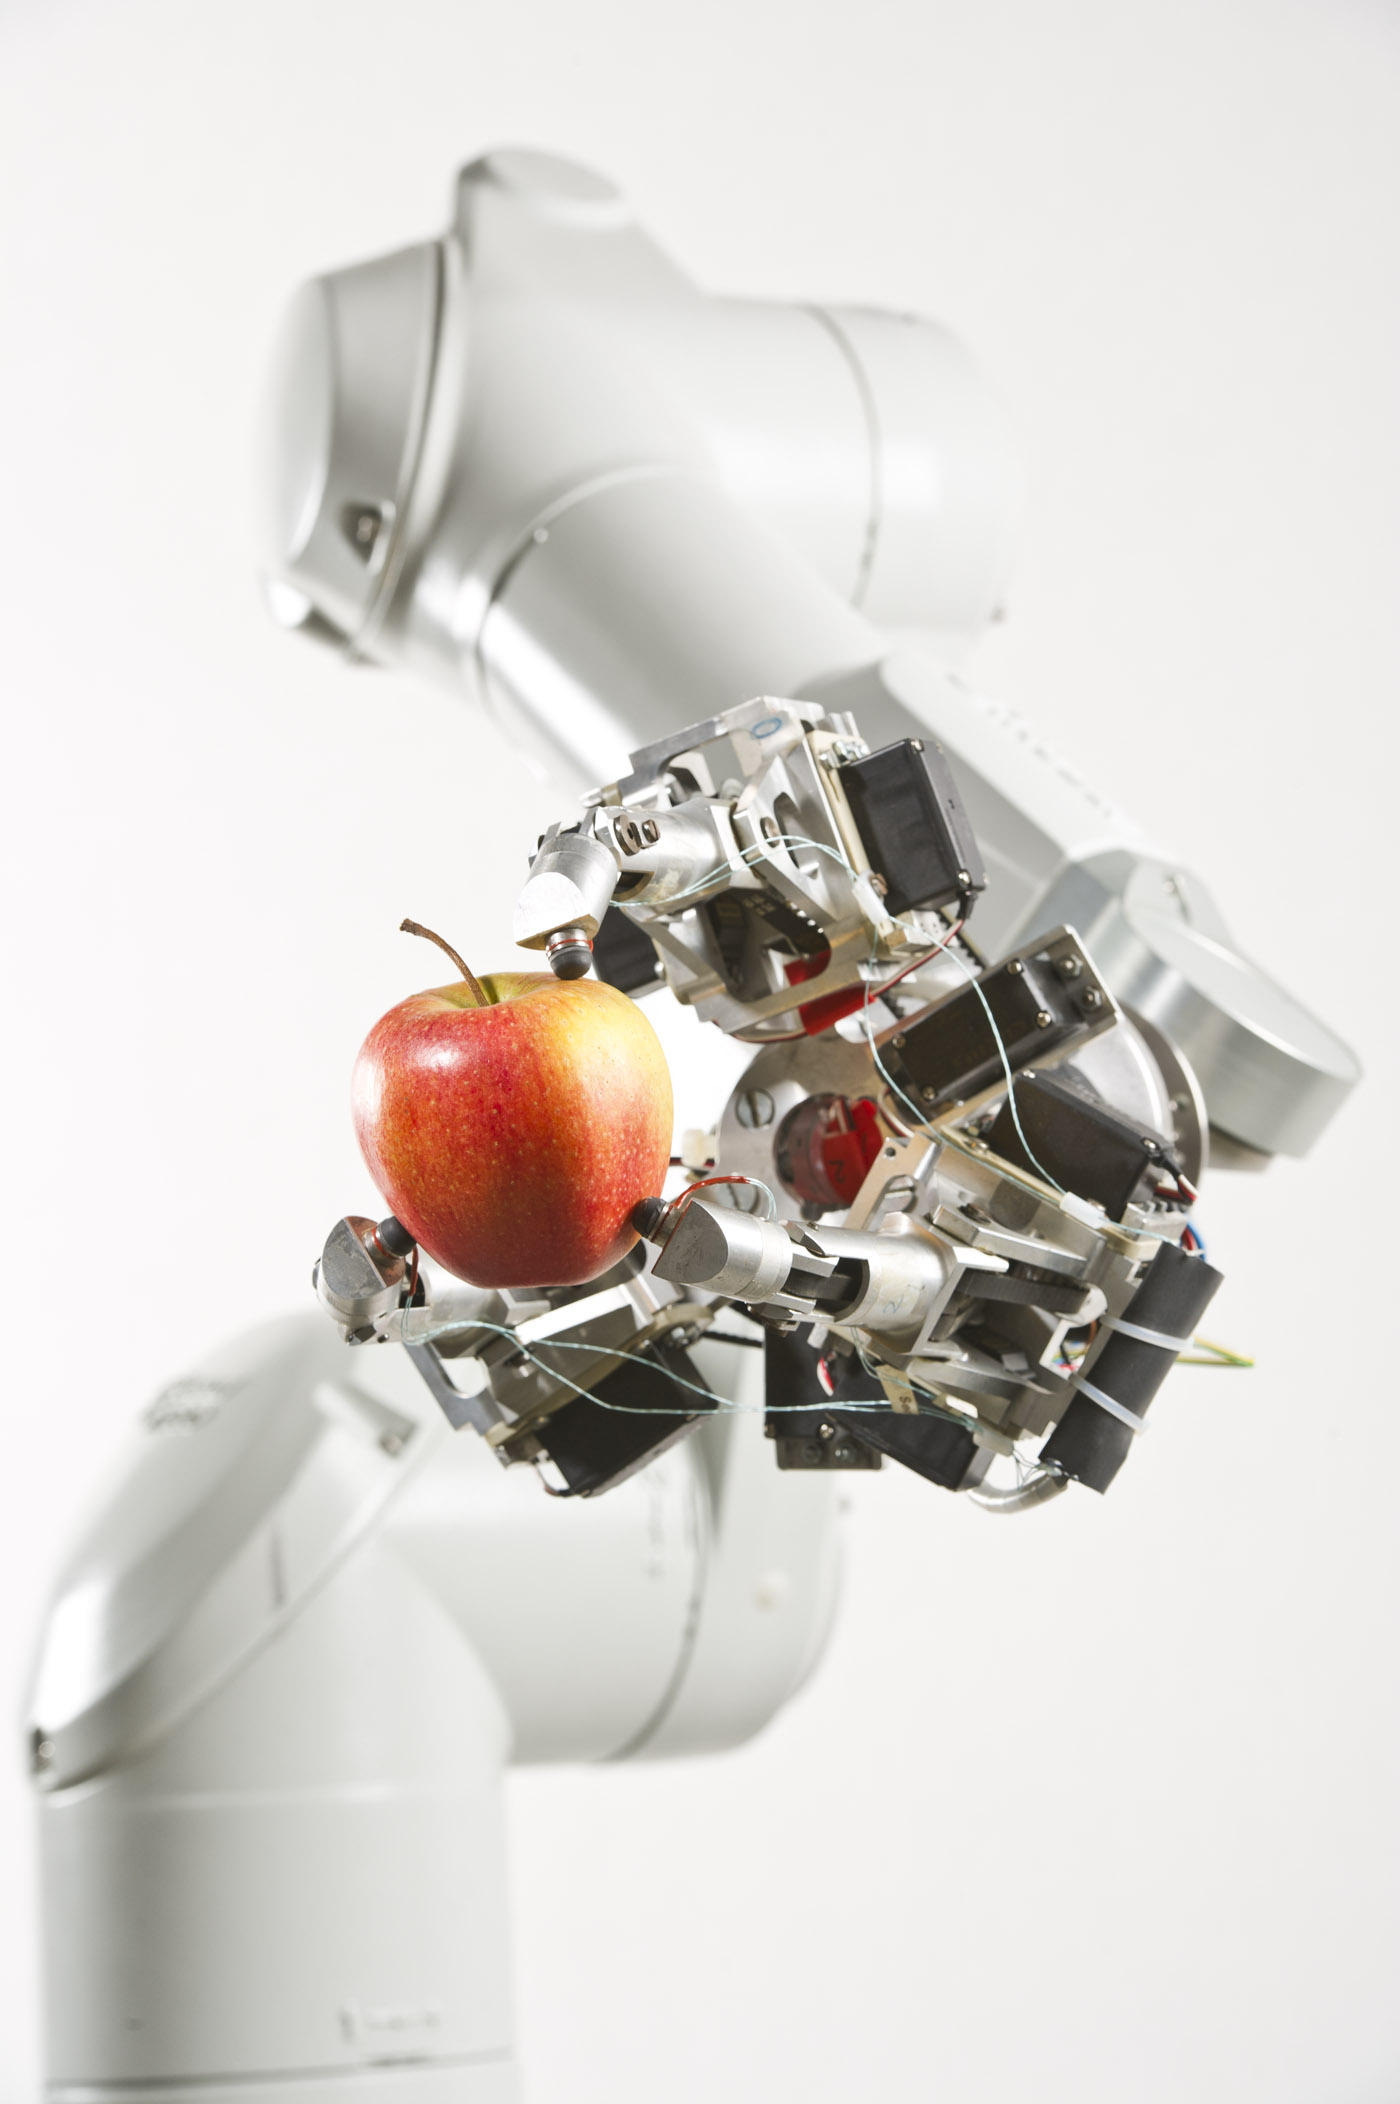
\includegraphics[height=\pictureheight]{Biomechgreifer.jpg}
		\subcaption{Roboterhand mit Apfel}
		\label{Bild_Beispiel_zwei_Bilder_links}
	\end{minipage}
%	
	\begin{minipage}[c]{.49\textwidth}
    		\centering
		
\includegraphics[height=\pictureheight]{LogoFAPS}
		\subcaption{FAPS-Logo}
		\label{Bild_Beispiel_zwei_Bilder_rechts}
	\end{minipage}
    	
    	\caption[Zwei Bilder nebeneinander]{Hier sind zwei Bilder zu sehen, welche nebeneinander angeordnet sind.}
	\label{Bild_Beispiel_zwei_Bilder}

\end{figure}

Auflistungen werden wie folgt gemacht:
\begin{itemize}
	\item Das wird der erste Stichpunkt \\ \vspace{-1cm}
	\item Der zweite Stichpunkt ist mit $\backslash\!vspace\left\{ -1cm \right\}$ in vertikaler Richtung verschoben \\ \vspace{-1cm}
\end{itemize}


		% Folgender Befehl erzwingt an entsprechender Stelle einen Seitenumbruch
		% Bei einer Seite bitte ausblenden
%		\addtocontents{toc}{\protect\newpage}

		\chapter{Zusammenfassung und Ausblick}
Für das Durchhalten des Lesers lobende Worte....


	%%%%%%%%%%%%%%%%%%%%%%%%%%%%%%%%%%%%%%%%%%%%%%%%%%%%%%%%%%%%%%%%%%%%%%%%%%%%%%%%%%%%%%%%%%%%%
	%%%   NICHT AENDERN!!!                                                                    %%%
	%%%%%%%%%%%%%%%%%%%%%%%%%%%%%%%%%%%%%%%%%%%%%%%%%%%%%%%%%%%%%%%%%%%%%%%%%%%%%%%%%%%%%%%%%%%%%
	
	\cleardoublepage
\thispagestyle{plain}

% Inhaltsverzeichnis-Eintrag
% Text des Labels beginnt im Abstand von x.xem vom linken Rand
\titlecontents{chapter}[0.0em]{%
}{% Nummerierung vom Textbeginn um x.xem nach links verschieben
\contentslabel{0.0em}
}{%
}{% Abstand der Zeichen hinter Kapitelname + Seitenangabe
\titlerule*[0.7725pc]{.}\contentspage
}

\phantomsection
\addcontentsline{toc}{chapter}{Literaturverzeichnis}

% Am besten aus Citavi exportieren
\bibliography{Literatur}
% Literaturverzeichnis Stil
\bibliographystyle{is-abbrv}
%	Pfad:		C:\Program Files (x86)\MiKTeX 2.9\miktex\bin\bibtex.exe
%	Argumente:	"%bm"}

% Layout Inhaltsverzeichnis wiederherstellen
% Inhaltsverzeichnislayout
\setcounter{tocdepth}{3} % 3 Gliederungsebenen im Inhaltsverzeichnis

% Text des Labels beginnt im Abstand von x.xem vom linken Rand
\titlecontents{chapter}[1.0em]{%
}{% Nummerierung vom Textbeginn um x.xem nach links verschieben
\contentslabel{1.0em}
}{%
}{% Abstand der Zeichen hinter Kapitelname + Seitenangabe
\titlerule*[0.7725pc]{.}\contentspage
}

% Sections
% Text des Labels beginnt im Abstand von x.xem vom linken Rand
\titlecontents{section}[3.133em]{%
}{% Nummerierung vom Textbeginn um x.xem nach links verschieben
\contentslabel{1.809em}
}{%
}{% Abstand der Zeichen hinter Kapitelname + Seitenangabe
\titlerule*[0.7725pc]{.}\contentspage
}

% Subsections
\titlecontents{subsection}[6.067em]{%
%\addvspace{-0.5pc}
}{% Nummerierung vom Textbeginn um x.xem nach links schieben
\contentslabel{2.605em}
}{% Nach dem Label
}{% Abstand der Zeichen hinter Kapitelname + Seitenangabe
\titlerule*[0.7725pc]{.}\contentspage
}

% Zu Testzwecken: Naechste Zeile in vorherige Zeile schieben
%\addvspace{-1.941pc}\color{red}


% Abbildungs- und Tabellenverzeichnis Formatierung
\makeatletter
\renewcommand*{\l@figure}{\@dottedtocline{1}{0.0em}{2.5em}}
\renewcommand*{\l@table}{\@dottedtocline{1}{0.0em}{2.5em}}
\makeatother

% Abstand zwischen Ueberschriften und dem ersten Eintrag der toc, lof, lot 
\setlength{\cftaftertoctitleskip}{3.85em}
\setlength{\cftafterloftitleskip}{3.85em}
\setlength{\cftafterlottitleskip}{3.85em}	% Literaturverzeichnis (BibTeX)	
	
	\appendix										% Beginn des Anhangs
	
% Bezeichnungen und Nummerierungsstile
\renewcommand{\chaptername}{Anhang}
% \renewcommand{\theequation}{\Alph{section}.\arabic{equation}}
\renewcommand{\theequation}{\Alph{chapter}.\arabic{equation}}
\renewcommand{\thetable}{\Alph{section}.\arabic{table}}
\renewcommand{\thefigure}{\Alph{section}.\arabic{figure}}


% Inhaltsverzeichnislayout fuer 'Anhang'
% Text des Labels beginnt im Abstand von x.xem vom linken Rand
\titlecontents{chapter}[0.0em]{%
}{% Nummerierung vom Textbeginn um x.xem nach links verschieben
\contentslabel{0.0em}
}{%
}{% Abstand der Zeichen hinter Kapitelname + Seitenangabe
\titlerule*[0.7725pc]{} % \contentspage
}

% Erscheinen von 'Anhang' im Inhaltsverzeichnis
\addtocontents{toc}{\protect\contentsline{chapter}{Anhang}{}{}}

% Layout Inhaltsverzeichnis wiederherstellen
% Inhaltsverzeichnislayout
\setcounter{tocdepth}{3} % 3 Gliederungsebenen im Inhaltsverzeichnis

% Text des Labels beginnt im Abstand von x.xem vom linken Rand
\titlecontents{chapter}[1.0em]{%
}{% Nummerierung vom Textbeginn um x.xem nach links verschieben
\contentslabel{1.0em}
}{%
}{% Abstand der Zeichen hinter Kapitelname + Seitenangabe
\titlerule*[0.7725pc]{.}\contentspage
}

% Sections
% Text des Labels beginnt im Abstand von x.xem vom linken Rand
\titlecontents{section}[3.133em]{%
}{% Nummerierung vom Textbeginn um x.xem nach links verschieben
\contentslabel{1.809em}
}{%
}{% Abstand der Zeichen hinter Kapitelname + Seitenangabe
\titlerule*[0.7725pc]{.}\contentspage
}

% Subsections
\titlecontents{subsection}[6.067em]{%
%\addvspace{-0.5pc}
}{% Nummerierung vom Textbeginn um x.xem nach links schieben
\contentslabel{2.605em}
}{% Nach dem Label
}{% Abstand der Zeichen hinter Kapitelname + Seitenangabe
\titlerule*[0.7725pc]{.}\contentspage
}

% Zu Testzwecken: Naechste Zeile in vorherige Zeile schieben
%\addvspace{-1.941pc}\color{red}


% Abbildungs- und Tabellenverzeichnis Formatierung
\makeatletter
\renewcommand*{\l@figure}{\@dottedtocline{1}{0.0em}{2.5em}}
\renewcommand*{\l@table}{\@dottedtocline{1}{0.0em}{2.5em}}
\makeatother

% Abstand zwischen Ueberschriften und dem ersten Eintrag der toc, lof, lot 
\setlength{\cftaftertoctitleskip}{3.85em}
\setlength{\cftafterloftitleskip}{3.85em}
\setlength{\cftafterlottitleskip}{3.85em}				% Formatierung des Anhangs
		
	%%%%%%%%%%%%%%%%%%%%%%%%%%%%%%%%%%%%%%%%%%%%%%%%%%%%%%%%%%%%%%%%%%%%%%%%%%%%%%%%%%%%%%%%%%%%%
	%%%   MIT INHALT ZU FUELLEN                                                               %%%
	%%%%%%%%%%%%%%%%%%%%%%%%%%%%%%%%%%%%%%%%%%%%%%%%%%%%%%%%%%%%%%%%%%%%%%%%%%%%%%%%%%%%%%%%%%%%%

%
%	Das Einfuegen des Anhangs erfolgt hier
%

		\chapter{Titel des Anhangs A}
\label{Anhang_A}
% 
Hier kommt das hin, was in der Ausführung für Unübersichtlichkeit gesorgt
hätte...

	
	
	%%%%%%%%%%%%%%%%%%%%%%%%%%%%%%%%%%%%%%%%%%%%%%%%%%%%%%%%%%%%%%%%%%%%%%%%%%%%%%%%%%%%%%%%%%%%%
	%%%   NICHT AENDERN!!!                                                                    %%%
	%%%%%%%%%%%%%%%%%%%%%%%%%%%%%%%%%%%%%%%%%%%%%%%%%%%%%%%%%%%%%%%%%%%%%%%%%%%%%%%%%%%%%%%%%%%%%
	
	\ifthenelse{\equal{\Lebenslauf}{CV}}{
		\cleardoublepage

\chapter*{Curriculum Vitae}

\thispagestyle{empty}

Hier erscheint bei Masterarbeiten der Lebenslauf...
		\currentpdfbookmark{Curriculum Vitae}{Curriculum Vitae}	% Lesezeichen fuer Lebenslauf
	}{}


\end{document}